% !TEX root = ../main.tex
\chapter{Applications of Linear Second Order Equations}
\chapterdate{10/25--10/28}

\section{Vibrating Springs}

We consider the motion of an object with mass attached to an end of a spring with negligible mass that is vertically attached to a fixed object.

The spring–mass system is in \emph{\textbf{equilibrium}} when the object is at rest and the forces acting on it sum to zero. The position of the object in this case is the \emph{\textbf{equilibrium position}}. 

Denote by $y$ the displacement of the object from its equilibrium position at time $t$, measured positive upward.

\begin{figure}[htb]
\centering
  \begin{tikzpicture}
    \node[rectangle,fill=yellow!60,draw=black!90,inner sep=2.5mm, anchor=north] (a) at (0,4) {$m$};
    \node[rectangle,fill=yellow!60,draw=black!90,inner sep=2.5mm, anchor=north] (b) at (3,2) {$m$};
    \node[rectangle,fill=yellow!60,draw=black!90,inner sep=2.5mm, anchor=north] (c) at (6,0) {$m$};
    \draw[
        decoration={
            coil,
            aspect=0.3, 
            segment length=1mm, 
            amplitude=3mm,
            pre length=2mm,
            post length=2mm
        },
        decorate
    ] (0,6) -- (a); 
    \draw[
        decoration={
            coil,
            aspect=0.3, 
            segment length=2mm, 
            amplitude=3mm,
            pre length=2mm,
            post length=2mm
        },
        decorate
    ] (3,6) -- (b); 
    \draw[
        decoration={
            coil,
            aspect=0.3, 
            segment length=3mm, 
            amplitude=3mm,
            pre length=2mm,
            post length=2mm
        },
        decorate
    ] (6,6) -- (c); 
    \fill [pattern = north east lines] (-1,6) rectangle (1, 6.2);
    \draw[thick] (-1,6) -- (1,6);
    \fill [pattern = north east lines] (2,6) rectangle (4,6.2);
    \draw[thick] (2,6) -- (4,6);
    \fill [pattern = north east lines] (5,6) rectangle (7,6.2);
    \draw[thick] (5,6) -- (7,6);
    \draw[-latex,thick,blue] (-2,-1) -- (-2,6) node[anchor=south] {$y$};

    \node[
      left,
      red, 
      label={
          [red]left:{
            \parbox{\widthof{Equilibrium}}{\centering Equilibrium \\ position}
            }
        }
    ] (o) at (-2,2) {$0$};

    \draw[dashed, blue] (a.north)--coordinate[midway](am) (-2, 4); 
    \draw[dashed, red] (b.north)--coordinate[midway](bm) (-2, 2) coordinate(b1); 
    \draw[dashed, blue] (c.north)--(-2, 0);
    \draw[latex-latex] (am)--++(0,-2) node[midway,right]{$y>0$};
    \draw[latex-latex] (bm)--++(0,-2) node[midway, left]{$y<0$};
    \end{tikzpicture}
    
    \caption{Spring-mass system}
\end{figure}


\href{https://en.wikipedia.org/wiki/Hooke\%27s_law}{Hooke's Law - Wikipedia} says that if the length of the spring is changed by an amount $\Delta L$ from its natural length, if it is then the spring exerts a force $F_s$ whose magnitude that is proportional to $\Delta L$, that is $|F_s|=k\Delta L$, where $k$ is a positive number called the spring constant. Since we take upward as the positive direction, the force is  $F_s=k\Delta L$ if the spring is stretched or $F_s=-k\Delta L$ if the spring is compressed.,


\begin{figure}[htb]
\centering
  \begin{tikzpicture}
    \draw[
        decoration={
            coil,
            aspect=0.3, 
            segment length=1mm, 
            amplitude=3mm,
            pre length=2mm,
            post length=2mm
        },
        decorate
    ] (0,4)coordinate(a1) -- (0,1.5)coordinate(a2);
    
    \draw[
        decoration={
            coil,
            aspect=0.3, 
            segment length=1.5mm, 
            amplitude=3mm,
            pre length=2mm,
            post length=2mm
        },
        decorate
    ] (3,4)coordinate(b1) -- (3,0)coordinate(b2);
    \node[rectangle,fill=yellow!60,draw=black!90,inner sep=2.5mm, anchor=north] at (b2) {$m$};
    
    \fill [pattern = north east lines] ($(a1)+(-1,0)$) rectangle ($(a1)+(1, 0.2)$);
    \draw[thick] ($(a1)+(-1,0)$) -- ($(a1)+(1,0)$);

    \fill [pattern = north east lines] ($(b1)+(-1,0)$) rectangle ($(b1)+(1, 0.2)$);
    \draw[thick] ($(b1)+(-1,0)$) -- ($(b1)+(1,0)$);

    \draw[
      latex-latex,
      red
    ] (a1)++(-0.75,0)--($(a2)+(-0.75,0)$)
      node[
        midway, 
        shape=rectangle, 
        fill=white, 
        label={
          [red]left:{\small Natural length}
        }
      ]{$L$};

    \draw[
      latex-latex, 
      blue, 
      shift={(-0.5,0)}
    ] ($(a2)!0.5!(b2|-a2)$)coordinate(ab)--($(b2)!0.5!(a2|-b2)$) 
      node[
        midway, 
        shape=rectangle, 
        fill=white, 
        label={[blue]left:{\small Change in length}
        }
      ] {$\Delta L$};

    \draw[dashed] ($(a2)+(-1,0)$)--($(ab)+(1,0)$);
    \draw[dashed] (a2|-b2)--(b2);
    \draw[
      -latex, 
      color=blue
    ] (b2)++(1, 0)--++(0,2) 
      node[
        midway, 
        right
      ] {$F_s=k\Delta L$}; 
    % \draw[-latex, color=blue!60] (b2)++(1, 0)--++(0,-2) node[midway, right] {$F_g=-mg$};  
    \end{tikzpicture}
    
    \caption{Hooke's Law of Spring}
\end{figure}


Besides Earth's gravitational force and the force of the spring, there can be other forces.
The system may have a damping force $F_d=-cy'$ that resists the motion with a force proportional to the velocity of the object. 
It may be due to resistance or friction. 
We say that the motion is \emph{\textbf{undamped}} if $c=0$, or \emph{\textbf{damped}} if $c>0$.

\begin{figure}[htb]
  \centering
    \begin{tikzpicture}
      \draw[
          decoration={
              coil,
              aspect=0.3, 
              segment length=1mm, 
              amplitude=3mm,
              pre length=5mm,
              post length=10mm
          },
          decorate
      ] (0,5)coordinate(a1) -- (0,1)coordinate(a2);
      \node[rectangle,fill=yellow!60,draw=black!90,inner sep=2.5mm, anchor=north] at (a2) {$m$};

      \fill [pattern = north east lines] ($(a1)+(-1,0)$) rectangle ($(a1)+(1, 0.2)$);
      \draw[thick] ($(a1)+(-1,0)$) -- ($(a1)+(1,0)$);

      % \begin{pgfonlayer}{background}

      \draw[ultra thick, double, double distance=1mm, double=gray, rounded corners=2pt] (a2)++(-0.75,0.75)coordinate(mul)--+(0,-2)coordinate(mll)--(mll)-|($(a2)+(0.75,0.75)$)--($(a2)+(0.75,0.75)$)coordinate(mur);
      
      \fill [pattern = north east lines, pattern color=cyan!60] ($(mll)+(0.1,0.1)$) rectangle ($(mur)+(-0.1, -0.25)$);
    % \end{pgfonlayer}
    \end{tikzpicture}
      
      \caption{A spring system with damping}
  \end{figure}

It may have an external force $F$, other than the force due to gravity, that may vary with $t$, but is independent of displacement and velocity. We say that the motion is \emph{\textbf{free}} if $F\equiv0$, or \emph{\textbf{forced}} if $F\not\equiv0$.

By Newton’s second law of motion, we have
\[ma=-mg+F_d+F_s+F=-mg-cy'+F_s+F,\]
where $a=y''$ is the acceleration.

Let $\Delta l$ be the change of length when the system reaches equilibrium. Then $mg=k\Delta l$. When the displacement of the object is $y$, the change in length of the spring is $|y-\Delta l|$ and $F_s=k(\Delta l - y)$.  

Therefore, 
\[-mg+F_s = -ky.\]

\begin{figure}[htb]
  \centering
    \begin{tikzpicture}
      % Spring left
      \node[rectangle,fill=yellow!60,draw=black!90,inner sep=2.5mm, anchor=north] (a) at (0,4) {$m$};
      \draw[
          decoration={
              coil,
              aspect=0.3, 
              segment length=1mm, 
              amplitude=3mm,
              pre length=2mm,
              post length=2mm
              },
              decorate
      ] (0,6)coordinate(m1) -- (a);
      \draw[thick] ($(m1)+(-1,0)$) -- ($(m1)+(1,0)$);
      \fill [pattern = north east lines] ($(m1)+(-1,0)$) rectangle ($(m1)+(1,0.2)$);
              
      % Spring middle 
      \draw[
          decoration={
              coil,
              aspect=0.3, 
              segment length=2mm, 
              amplitude=3mm,
              pre length=2mm,
              post length=2mm
          },
          decorate
      ] (4,6)coordinate(m0) -- (4,2) coordinate(b);
      \draw[thick] ($(m0)+(-1,0)$) -- ($(m0)+(1,0)$);
      \fill [pattern = north east lines] ($(m0)+(-1,0)$) rectangle ($(m0)+(1,0.2)$);
      
      % Spring right
      \node[rectangle,fill=yellow!60,draw=black!90,inner sep=2.5mm, anchor=north] (c) at (8,0.5) {$m$};
      \draw[
          decoration={
              coil,
              aspect=0.3, 
              segment length=3mm, 
              amplitude=3mm,
              pre length=2mm,
              post length=2mm
          },
          decorate
      ] (8,6)coordinate(m2) -- (c);
      \draw[thick] ($(m2)+(-1,0)$) -- ($(m2)+(1,0)$);
      \fill [pattern = north east lines] ($(m2)+(-1,0)$) rectangle ($(m2)+(1,0.2)$);  

      % Vertical axis
      \draw[-latex,thick,blue] (-2,-2) -- (-2,6) node[anchor=east] {$y$};
    
      % level line natural spring (middle)
      \draw[dashed] ($(b.north)+(-3,0)$)coordinate(bnl)--($(b.north)+(2,0)$) coordinate(bnr);
      
      %level line compressed spring
      \draw[dashed, blue] (a.north-|bnl)++(1,0)--coordinate[midway](aR) (a.north) -- coordinate[midway](aL) (-2,4); 

      % equilibrium position
      \draw[dashed, red] (c.north)--(-2,0.5)coordinate(e);
      \node[
        left,
        red, 
        label={
            [red]left:{
              \parbox{\widthof{Equilibrium}}{\centering Equilibrium \\ position}
              }
          }
      ] at (e) {$0$};

      % change in length in Equilibrium State
        \draw[latex-latex, color=red] ([xshift=-0.5cm]bnr)--([xshift=-0.5cm]bnr|-c.north) node[midway,shape=rectangle, fill=white]{$\Delta l$};

      % change in length when compressed
      \draw[latex-latex, color=blue] ([xshift=0.5cm]aR)--([xshift=0.5cm]aR|-b.north) node[midway,shape=rectangle, fill=white]{$\Delta L$};

      % displacement y
      \draw[latex-latex, color=blue] (aL)--(aL|-c.north) node[midway,shape=rectangle, fill=white,xshift=2mm]{$y={\color{red}\Delta l} + \Delta L$};

      % label natural length
      \draw[latex-latex] ([xshift=0.8cm]b.north)--++(0, 4) node[midway,shape=rectangle, fill=white, rotate=-90]{\small Natural Length $L$};

      % Spring force left
      \draw[latex-, color=blue]
        (a.north)++(0.8, 0.5)--++(0,1) 
      node[
        midway,
        % xshift=0.2cm,
        right
        % rotate=-90
      ] {$\begin{aligned}{F_{s_c}}=&{\color{red}-}k\Delta L\\ =&k(\Delta l-y)\end{aligned}$}; 

      % Spring force right
      \draw[-latex, color=red]
        ($(c.north)+(0.8, 2.5)$)coordinate(f)--coordinate[midway](cfs)++(0,0.8);
      \node[
        % xshift=0.2cm,
        right, 
        text=red
        % rotate=-90
      ] (fs) at (cfs) {$F_{s_e}=k\Delta l$};

      % gravity right
      \draw[-latex, color=blue]
        (f)--coordinate[midway](cfg)++(0,-0.8); 
      \node[
        % xshift=0.2cm,
        right,
        text=blue
        % rotate=-90
      ] (fg) at (cfg) {$F_{g}=-mg$};

      \node[right] (p) at ($(cfs)!0.5!(cfg)$) {$+$};
      \node[above, rotate=-90] at ([yshift=-0.4cm]cfg) {$=$};
      \node[right] at ([yshift=-0.8cm]cfg) {$0$};
      \end{tikzpicture}
      
      \caption{Relation between displacement and change in length}
  \end{figure}

So the displacement $y$ of a object attached to a spring satisfies the following equation
\begin{equation}
  y''+\frac{c}{m}y'+\frac{k}{m}y=\frac{F(t)}{m}.\label{eq:VSpringMotion}
\end{equation}

Note that for a horizontal spring motion, Equation \eqref{eq:VSpringMotion} is still valid.

\subsection{Simple harmonic motion}
Assume there is no damping force or other external force, that is, $F_d\equiv 0$ and $F\equiv 0$. Then, by Newton's second law of motion, the displacement $y$ satisfies the following equation
\[y''+\frac{k}{m}y=0.\]
This motion is known as the \emph{\textbf{simple harmonic motion}}.

Let $\omega=\sqrt{\frac km}$. Then the general solution of the equation $my'+ky=0$ is
\[y=C_1\cos(\omega t)+C_2\sin(\omega t).\]
If further, we let $R=\sqrt{\left(C_1\right)^2+\left(C_2\right)^2}$ and  $\phi$ the angle in $(-\pi,\pi)$ such that $\cos\phi=\frac{C_1}{R}$ and $\sin\phi=-\frac{C_2}{R}$, then the general solution can be written as
\[y=R\cos(\omega t+\phi).\]
Here, the angle $\phi$ is known as the \emph{\textbf{phase angle}},  $R$ is the amplitude of the oscillation and the solution $y=R\cos(\omega t+\phi)$ is called the \emph{\textbf{amplitude-phase form}} of the displacement. The constant $\omega$ is the \emph{\textbf{frequency}} of the motion. If the time $t$ is measured in seconds, then, the frequency is measured in cycle per second or, in international unit, Hertz (Hz for short). Because the \emph{\textbf{period}} $T$ of the amplitude-phase form displacement is 
\[T=\frac{2\pi}{\omega}.\]

\begin{example}
An object stretches a spring \SI{5}{\meter} in equilibrium.
\begin{enumerate}
  \item 
  Find the displacement of the object after $t$ seconds if it is initially displaced \SI{18}{\meter} above equilibrium and given a downward velocity of \SI{7}{\meter\per\second}.
  \item Find the frequency, amplitude, the phase angle of this motion, and the amplitude-phase form of the displacement.
\end{enumerate}
\end{example}
\begin{solution}
  \begin{enumerate}
    \item 
  The motion of the object is undamped and free, that is $F_d\equiv 0$ and $F\equiv 0$. So the displacement $y$ away from the equilibrium position satisfies the differential equation
  \[y''+\frac{k}{m}y=0,\]
  where $m$ is the mass and $k$ is the spring constant.

  Since the spring stretches \SI{5}{\meter} to reach the equilibrium position, the spring constant $k$ is determined by the equation
  \[mg=k\cdot 6.\]

  Since the units for the displacement is in meters, we take the gravitational acceleration to be $g=\SI{9.8}{\meter\square\per\second}$ and then
  \[\frac{k}{m}=\frac{9.8}{5}=\frac{49m}{25}.\]

  Therefore, the displacement $y$ satisfies
  \[
  \begin{aligned}
    my''+\frac{49m}{25}y=&0\\
    y''+\frac{49}{25}y=&0.
  \end{aligned}  
  \]

The associated characteristic equation $r^2+\frac{49}{25}=0$ has two complex solutions $r=\pm\frac{7\mathrm{i}}{5}$. Therefore, the general solution is
\[y=C_1\cos\left(\frac{7}{5}t\right)+C_2\sin\left(\frac{7}{5}t\right).\]

Because the object is initially displaced \SI{18}{\meter} above equilibrium and given a downward velocity of \SI{7}{\meter\per\second}. In terms of mathematical equalities, we have
\[y(0)=18\qquad\text{and}\qquad y'(0)=-7.\]
Note that 
\[y'=-\frac{7}{5}C_1\sin\left(\frac{7}{5}t\right)+\frac{7}{5}C_2\cos\left(\frac{7}{5}t\right)\]
Then $C_1=18$, $C_2=-5$, and the displacement $y$ at time $t$ is
\[y=18\cos\left(\frac{7}{5}t\right)-5\sin\left(\frac{7}{5}t\right)\quad \si{\meter}.\]

\item The frequency is $\omega=\frac{7}{5} \si{\radian\per\second}$.

The amplitude is
\[R=\sqrt{18^2+(-5)^2}=\sqrt{349} \si{\radian\per\second}.\]

Since 
\[
\begin{aligned}
  \cos\phi=&\frac{C_1}{R}=\frac{18}{\sqrt{18^2+(-5)^2}}=\frac{18}{\sqrt{349}}\\
  \sin\phi=&\frac{-C_2}{R}=-\frac{-5}{\sqrt{18^2+(-5)^2}}=\frac{5}{\sqrt{349}}\\
  \tan\phi=&\frac{-C_2}{C_1}=\frac{5}{18},
\end{aligned}  
\]
the angle $\phi$ is in the first quadrant, and 
\[\phi= \arctan\left(\frac{5}{18}\right) \si{\radian}.\]

The amplitude-phase form of the displacement is about
\[y=\sqrt{349}\cos\left(\frac75t + \arctan\left(\frac{5}{18}\right)\right)~\si{\meter}.\]
\end{enumerate}
\end{solution}

\begin{exercise}
  The natural length of a spring is \SI{1}{\meter}. An object is attached to it and the length of the spring increases to \SI{1.2}{\meter} when the object is in equilibrium. Then the object is initially displaced downward \SI{0.4}{\meter} and given an upward velocity of \SI{2.1}{\meter\per\second}. Find the amplitude-phase form of the displacement for $t>0$.
\end{exercise}
\begin{exersol}
Since the gravitational acceleration is $g=\SI{9.8}{\meter\per\square\second}$ and the change in length at the equilibrium position is $\Delta l=1.2-1=0.2~\si{\meter}$, the ratio of the spring constant and the mass is  
\[\frac{k}{m}=\frac{g}{\Delta l}=\frac{9.8}{0.2}=49,\]
and the frequency is
\[\omega=\sqrt{\frac{k}{m}}=\sqrt{49}=\SI{7}{\Hz}.\] 

Therefore, the displacement $y$ satisfies the initial value problem
\[y'' + 49y=0, \quad y(0)=-0.4,\quad y'(0)=1.4.\]
The general solution of the differential equation is
\[y=C_1\cos(\omega t)+C_2\sin(\omega t) = C_1\cos(7t)+C_2\sin(7t).\]
So
\[y'=-7C_1\sin(7t)+7C_2\cos(7t).\]
Substituting the initial conditions into $y$ and $y'$ yields $C_1=-0.4$ and $C_2=0.3$. Hence, the displacement is
\[y=-0.4\cos(7t)+0.3\sin(7t)\]

The amplitude is
\[R=\sqrt{\left(C_{1}\right)^{2}+\left(C_{2}\right)^{2}}=\sqrt{(-0.4)^2+0.3^2}=0.5\]

The phase angle is determined by
\[\cos\phi = \frac{C_{1}}{R}=\frac{-0.4}{0.5}=-\frac45\quad\text{and}\quad \sin\phi = -\frac{C_{2}}{R}=-\frac{0.3}{0.5}=-\frac35.\]
Therefore, $\phi$ is in the third quadrant and
\[\phi = -\arccos\left(-\frac45\right)\text{rad}.\]

So the amplitude-phase form of the displacement is
\[y=0.5\cos(7t-0.64).\]
\end{exersol}

\section{Free Vibrations with Damping}
Assume that the damping force is proportional to the velocity of the mass and acts in the direction opposite to the motion, that is
\[F_d=-cy',\]
where $c$ is a positive constant, called the damping constant. Then the displacement satisfies the equation
\[y''+\frac{c}{m}y'+\frac{k}{m}y=0.\]
The solution of this equation depends on the value of $c$, or more precisely, the value of $\sqrt{c^2-4km}$. The reason is that the associated characteristic equation 
\[r^2+\frac{c}{m}r+\frac{k}{m}=0,\]
whose solutions
$r=\frac{-c\pm\sqrt{c^2-4km}}{2m}$
may be two complex roots, a double root, or two distinct real roots.

\subsection*{Underdamping} 

The motion is said to be \emph{\textbf{underdamped}}, if $c^2<4mk$. In this case, the solutions are complex roots 
\[r=\frac{-c\pm\sqrt{c^2-4mk}}{2m}=\frac{-c\pm\mathrm{i}\sqrt{4mk-c^2}}{2m}.\] 
Let $\omega_1=\frac{\sqrt{4mk-c^2}}{2m}$. Then the general solution is
\[y=e^{-\frac{ct}{2m}}(C_1\cos(\omega_1 t) + C_2\sin(\omega_1 t)).\]
Again, we may derive an amplitude-phase form of the displacement
\[y=Re^{-\frac{ct}{2m}}\cos(\omega_1 t +\phi),\]
where
\[R=\sqrt{C_1^2+C_2^2},\qquad \cos\phi=\frac{C_1}{R},\qquad \sin\phi=-\frac{C_2}{R},\qquad -\phi<\phi<\pi.\]
In the amplitude-phase form of the displacement, the factor $Re^{-\frac{ct}{2m}}$ is called the \emph{\textbf{time–varying amplitude}} of the motion, the quantity $\omega_1$ is called the \emph{\textbf{frequency}}, and $T=\frac{2\pi}{\omega_1}$ is called the \emph{\textbf{quasi–period}} of the displacement.

\begin{figure}[htb]
  \centering
  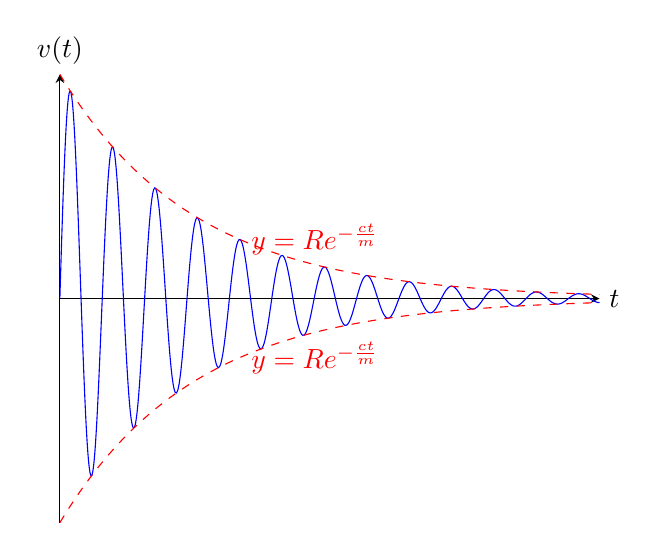
\begin{tikzpicture}
    \begin{axis}[
      domain=0:4,samples=501,axis lines=center,
      xtick=\empty,
      ytick=\empty,
      xlabel={$t$},
      xlabel style={anchor=west},
      ylabel={$v(t)$},
      ylabel style={anchor=south}
    ]
    \addplot[color=blue, smooth] {exp(-x)*sin(20*deg(x))};
    \addplot[color=red, dashed, smooth] {exp(-x)} node [pos=0.5, above] {$y=Re^{-\frac{ct}{m}}$};
    \addplot[color=red, dashed, smooth] {-exp(-x)} node [pos=0.5, below] {$y=Re^{-\frac{ct}{m}}$};
    \end{axis}
\end{tikzpicture}
\caption[Undamped motion]{Graph of the displacement of an undamped motion}
\end{figure}

\begin{example} 
	An object with mass \SI{2}{\kg} is hanging at one end of a spring with the spring constant $k=\SI{50}{\kg\per\square\second}$. The spring is subject to a damping force with the damping constant $c=\SI{12}{\kg\per\second}$. Suppose the object is initially displaced downward \SI{4}{\meter} with a downward velocity \SI{8}{\meter\per\second}. Find the displacement of the object.
\end{example}
\begin{solution}
If the time $t$ is measured in seconds, then from the given information, the displacement $y$, measured in meters, is the solution of the following initial value problem
\[2y''+ 12y'+50y=0, \qquad y(0)=-4,\qquad y'(0)=-8,\]
or equivalently
\[y''+6y'+25y, \qquad y(0)=-4,\qquad y'(0)=-8.\]
The characteristic equation
\[r^2+6r+25=0\]
has two complex solutions
\[r=\frac{-6\pm\sqrt{6^2-25^2}}{2\cdot 2}=-3\pm 4\mathrm{i}.\]
Therefore, the general solution is
\[y=e^{-3t}(C_1\cos(4t)+C_2\sin(4t)).\]
Since
\[y'=e^{-3t}((-3C_1+4C_2)\cos(4t)+(-4C_1-3C_2)\sin(4t)),\]
plugging the initial conditions into $y$ and $y'$ yields
\[C_1=-4\qquad\text{and}\qquad C_2=-5.\]
So the displacement $y$ is given by
\[y=-e^{-5t}(4\cos(4t)+5\sin(4t)).\]
\end{solution}

\subsection*{Overdamping} 

The motion is said to be \emph{\textbf{overdamped}} if $c^2>4mk$. In this case, the solutions of the characteristic equation are distinct real roots 
\[r=\frac{-c\pm\sqrt{c^2-4mk}}{2m}.\]
The general solution is
\[y=C_1e^{\frac{\left(-c+\sqrt{c^2-4mk}\right)t}{2m}}+C_2e^{\frac{\left(-c-\sqrt{c^2-4mk}\right)t}{2m}}.\]

\begin{example} 
  An object with mass \SI{2}{\kg} is hanging at one end of a spring with the spring constant $k=\SI{50}{\kg\per\square\second}$. The spring is subject to a damping force with the damping constant $c=\SI{52}{\kg\per\second}$. Suppose the object is initially displaced \SI{6}{\meter} above the equilibrium position with a downward velocity \SI{30}{\meter\per\second}. Find the displacement of the object.
\end{example}
\begin{solution}
  If the time $t$ is measured in seconds, then from the given information, the displacement $y$, measured in meters, is the solution of the following initial value problem
  \[2y''+ 52y'+50y=0, \qquad y(0)=6,\qquad y'(0)=-30\]
  or equivalently
  \[y''+ 26y'+25y, \qquad y(0)=6,\qquad y'(0)=-30\]
  The characteristic equation
  \[r^2+26r+25=0\]
  has two real solutions
  \[r_1=-1\qquad\text{and}\qquad r_2=-25.\]
  Therefore, the general solution is
  \[y=C_1e^{-t}+C_2e^{-25t}.\]
  Since
  \[y'=-C_1e^{-t}-25C_2e^{-25t},\]
  plugging the initial conditions into $y$ and $y'$ yields
  \[C_1=5\qquad\text{and}\qquad C_2=1.\]
  So the displacement $y$ is given by
  \[y=5e^{-t}+e^{-25t}.\]
  \end{solution}

\subsection*{Critically Damping}
  
The motion is said to be \emph{\textbf{critically damped}} if $c=\sqrt{4mk}$. In this case $r_1=r_2=-\frac{c}{2m}$ and the general solution is
\[y=e^{-\frac{ct}{2m}}(c_1+c_2t).\]

\begin{example} 
An object with mass \SI{2}{\kg} is hanging at one end of a spring with the spring constant $k=\SI{50}{\kg\per\square\second}$. The spring is subject to a damping force with the damping constant $c=\SI{20}{\kg\per\second}$. Suppose the object is initially displaced \SI{1}{\meter} below the equilibrium position with a upward velocity \SI{3}{\meter\per\second}. Find the displacement of the object.
\end{example}
\begin{solution}
If the time $t$ is measured in seconds, then from the given information, the displacement $y$, measured in meters, is the solution of the following initial value problem
\[2y''+ 20y'+50y=0, \qquad y(0)=-1,\qquad y'(0)=3\]
or equivalently
\[y''+10y'+25y, \qquad y(0)=-1,\qquad y'(0)=3\]
The characteristic equation
\[r^2+10r+25=0\]
has a repeated root
\[r=-5.\]
Therefore, the general solution is
\[y=e^{-5t}(C_1+C_2 t).\]
Since
\[y'=e^{-5t}((-5C_1+C_2)-5C_2 t),\]
plugging the initial conditions into $y$ and $y'$ yields
\[C_1=-1\qquad\text{and}\qquad C_2=-2.\]
So the displacement $y$ is given by
\[y=-e^{-5t}-2te^{-5t}.\]
\end{solution}

\section{Forced vibrations}

Suppose that the motion of the spring is affected by an external force $F(t)$ depending on the time. Then the displacement $y$ satisfies the equation
\[my''+cy'+ky=F(t),\]
which is a non-homogeneous equation. 

\subsection*{Forced vibration without damping}

In many mechanical problems, a device is subjected to periodic external forces $F(t)$ but not damping, for example, $F(t)=F_0\cos(\omega_0t)$. In this case, the displacement of the object satisfies the equation
\[y''+\frac{k}{m}y=\frac{F_0}{m}\cos(\omega_0t).\]
If $\omega_0\neq \omega=\sqrt{\frac{k}{m}}$, solving this equation using the method of undetermined coefficients and using the identity $k=m\omega^2$ yields the general solution
\[y=C_1\cos(\omega t)+C_2\sin(\omega t)+\frac{F_0\cos(\omega_0 t)}{m(\omega^2-\omega_0^2)}.\] 

If $\omega_0=\omega$, the general solution is
\[
  \begin{aligned}
    y=&C_1\cos(\omega t)+C_2\sin(\omega t)+\frac{F_0t\sin(\omega t)}{2m \omega}\\
    =&C_1\cos(\omega t)+\left(C_2+\frac{F_0t}{2m \omega}\right)\sin(\omega t).
\end{aligned}
\]
In this case, the amplitude increases as time goes.
This phenomenon is known as the \emph{\textbf{resonance}}.

\begin{example}
  A \SI{2}{\kg} object is attached to a spring with constant $k = \SI{275}{\kg\per\second}$ and subjected to an external force $F(t)=32\cos{8t}~\si{\kg-\meter\per\square\second}$. The object begins at rest in its equilibrium position. Find its displacement for $t > 0$, with $y(t)$ measured positive upward.
\end{example}
\begin{solution}
  From the given information, the displacement satisfies
  \[2y''+128y=32\cos(8t),\qquad y(0)=0,\qquad y'(0)=0,\]
  equivalently,
  \[y''+64y=16\cos(8t),\qquad y(0)=0,\qquad y'(0)=0.\]
  Solving the equation by the method of undetermined coefficients yields the general solution to the homogeneous equation is 
  \[y(t)=C_1\cos(8t)+C_2\sin(8t)+t\sin(8t).\]
  Since $y(0)=0$ and $y'(0)=0$, the undetermined coefficients are
  \[C_1=0\qquad C_2=0.\]
  Therefore, the displacement is
  \[y=t\sin(8t).\]
\end{solution}

\subsection*{Forced vibrations with damping}

Suppose the damping constant $c$ is nonzero and the external force $F(t)=F_0\cos(\omega_0t)$. The general solution of the equation 
\[my''+cy'+ky=F_0\cos(\omega_0 t)\]
is in the form
\[y=y_h+y_p,\]
where $y_h$ is the general solution of the complementary equation and $y_p$ is a particular solution in the form
\[y_p=A\cos(\omega_0 t)+B\sin(\omega_0 t),\]
where $A$ and $B$ can be determined by plugging $y_p$ in the equation.

Differentiating $y_p$ yields
\[
  \begin{aligned}
    y_p'=&-A\omega\sin(\omega_0 t)+B\omega\cos(\omega_0 t).
    y_p'=&-A\omega^2\cos(\omega_0 t)-B\omega^2\sin(\omega_0 t).
  \end{aligned}
\]
Plugging them into $my''+cy'+ky$ yields
\[
  \begin{aligned}
    &my''+cy'+ky\\
    =&(-mA\omega_0^2+cB\omega_0+kA)\cos(\omega_0 t)+(-mB\omega_0^2-cA\omega_0+kB)\sin(\omega_0 t)
  \end{aligned}
\]
So $y_p$ is a particular solution if
\[
  \left\{
\begin{aligned}
  (k-m\omega_0^2)A+cB\omega_0=&F_0\\
  -cA\omega_0+(k-m\omega_0^2)B=&0.
\end{aligned} \right. 
\]

Solving $A$ and $B$ yields
\[
\begin{aligned}
  A=&\frac{(k-m\omega_0^2)F_0}{(k-m\omega_0^2)^2+c^2\omega_0^2}\\
  B=&\frac{(c\omega_0)F_0}{(k-m\omega_0^2)^2+c^2\omega_0^2}.
\end{aligned}
\]

Therefore,
\[
y_p=\frac{F_0}{(k-m\omega_0^2)^2+c^2\omega_0^2}\left[(k-m\omega_0^2)\cos\omega_0 t+c\omega_0\sin\omega_0 t\right]
\]
which can be written in the amplitude-phase form as
\[y_p=R\cos(\omega_0 t+\phi),\]
where 
\[R=\frac{F_0}{\sqrt{(k-m\omega_0^2)^2+c^2\omega_0^2}}\]
and the phase angle $\phi$ is determined by
\[\cos\phi=\frac{k-m\omega_0^2}{\sqrt{(k-m\omega_0^2)^2+c^2\omega_0^2}}\quad \text{and} \quad \sin\phi=-\frac{c\omega_0}{\sqrt{(k-m\omega_0^2)^2+c^2\omega_0^2}}.\]

When the motion is underdamped, that is,  $c^2<4km$, the general form of the displacement is
\[y=e^{-\frac{ct}{2m}}(C_1\cos(\omega_1t)+C_2\sin(\omega_1 t))+R\cos(\omega_0 t+\phi),\]
where $\omega_1=\frac{4km-c^2}{2m}$.

When the motion is overdamped, that is, $c^2>4km$, the general form of the displacement is
\[y=C_1e^{\frac{\left(-c+\sqrt{c^2-4mk}\right)t}{2m}}+C_2e^{\frac{\left(-c-\sqrt{c^2-4mk}\right)t}{2m}})+R\cos(\omega_0 t+\phi).\]

When the motion is critically damped, that is, $c^2=4km$, the general form of the displacement is
\[y=e^{-\frac{ct}{2m}}(C_1+C_2t)) + R\cos(\omega_0 t+\phi).\]

Since the exponential summand approaches to $0$ as $t$ goes to the infinity, for large $t$, the displacement $y$ is closely approximated by the particular solution $y_p$:
\[y\approx y_p=R\cos(\omega_0 t +\phi).\]

For this reason, we say that $y_h$ is the \emph{\textbf{transient component}} of the solution $y$, and $y_p$ is the \emph{\textbf{steady state component}} of $y$. Thus, for large $t$ the motion is like simple harmonic motion at the frequency of the external force.

An interesting question is to find the value of $\omega_0$ so that the amplitude of the steady state component is maximal. 
Let 
\[\rho(x)=(k-mx)^2+c^2x=m^2x^2+(c^2-2km)x+k^2,\qquad x\ge 0.\]
Then $R$ reaches its maximum $R_{\text{max}}$ when $\rho(\omega_0^2)$ attains its minimum.

If $c>\sqrt{2km}$, then the minimum of $\rho(\omega_0^2)$ is at $\omega_0=0$ and 
\[R_{\text{max}}=\frac{F_0}{k}.\]

If $c<\sqrt{2km}$, then the minimum of $\rho(\omega_0^2)$ is at 
\[\omega=\sqrt{\frac{2km-c^2}{2m^2}}\]
and
\[R_{\text{max}}=\frac{2mF_0}{c\sqrt{4km-c^2}}.\]


\begin{example} 
  A \SI{1}{\kg} object is attached to a spring with spring constant $k=\SI{8}{\kg\per\second}$, and subjected to an damping force with the constant $c=\SI{4}{\kg\per\second}$ and an external force $F(t)= 3 \cos (5t)~\si{\kg\meter\per\square\second}$. Find the general solution and also the steady periodic solution
\end{example}

\begin{solution}
  The displacement $y$ satisfies the equation
  \[y''+ 4y'+8y = 3\cos(5t).\]
 Solving the characteristic equation 
  \[\begin{aligned}
    r^2+4r+8=&0\\
    (r+2)^2+4=&0
  \end{aligned}
  \]
  yields
  \[r=-2\pm 2i.\]
  Then the general solution of the complementary equation is 
  \[y_h = e^{-2t} (C_1 \cos 2t + C_2 \sin 2t)\]
  
A particular solution can be taken in the form
  \[y_p = A\cos 5t + B\sin 5t,\]
  where $A$ and $B$ can be determined by the method of undetermined coefficients.
Differentiating $y_p$ yields
\[
\begin{aligned}
  y_p'=&5B\cos 5t -5A\sin 5t\\
  y_p'' =& -25A\cos 5t + -25B\sin 5t.
\end{aligned}
\]
Hence 
\[y_p''+ 4y_p'+8y_p = (-17A+20B)\cos 5t + (-17B-20A)\sin 5t.\]
For $y_p$ to be a solution, the above expression must equal to $3\cos(5t)$, which implies
  \[
    \left\{
  \begin{aligned}
    -17A+20B =& 3\\20A+17B=&0
  \end{aligned}\right.
  \]
Solving this system of equations yields
\[A= \frac{-51}{689}\qquad\text{and}\qquad B=\frac{60}{689}.\]

So the general solution is:
\[y = y_h + y_p = e^{-2t} (C_1 \cos 2t + C_2 \sin 2t) - \frac{51}{689}\cos 5t + \frac{60}{689}\sin 5t.\]

The steady periodic solution is
\[y=- \frac{51}{689}\cos 5t + \frac{60}{689}\sin 5t.\]

\end{solution}




